\documentclass{minimal}

\usepackage[compat=1.0.0]{tikz-feynman}

\begin{document}
\begin{equation}
\mathcal{M} =
    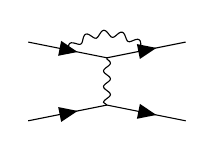
\begin{tikzpicture}[baseline=(c)]
        \begin{feynman}
            \vertex (a1) at (0, 0);
            \vertex (b1) at (.5, -.1);
            \vertex (c1) at (1, -.2);
            \vertex (d1) at (1.5, -.1);
            \vertex (e1) at (2, 0);
            \vertex (a2) at (0, -1);
            \vertex (c2) at (1, -.8);
            \vertex (e2) at (2, -1);
            \vertex (c) at (0, -.5);
            \diagram*{
                {[edges=fermion]
                (a1)--(c1)--(e1),
                (a2)--(c2)--(e2)},
                (b1) --[boson, quarter left] (d1),
                (c1) --[boson] (c2)
            };
        \end{feynman}
    \end{tikzpicture}
\end{equation}
\end{document}